\section{緒言}%===========================
エアシリンダは生産現場などに多く使われている.しかし,長いストロークを持ちつつも,コンパクトに使用するような場合には適合しない.よって,十分にストロークがありつつも,設置しやすい直動アクチュエータが求められている.
\par
そこで,曲げられるエアシリンダを開発する.本研究では曲げられるエアシリンダを"エアシリンダ型人工筋肉"と呼ぶ.エアシリンダ型人工筋肉は柔らかい素材で構成されている.そのため,曲がった状態で配置・動作し,高ストロークを有しつつもコンパクトに設置することができる.

しかし,エアシリンダ型人工筋肉は曲がった状態において,シリンダとロッドが接触する現象が起こる.本稿では,1つ目の内容として,シリンダを環状に巻き付けた状態における理論出力を導出し,実験値と比較する.
\par
2つ目の内容として,エアシリンダ型人工筋肉を機械要素として使用する際の制御特性について確認を行う.エアシリンダ型人工筋肉を揺動アームの機械要素とし,アームの角度制御とアーム先端のコンプライアンス制御を行い,制御性について評価を行う.
これら3つの内容を踏まえて,エアシリンダ型人工筋肉及びエアシリンダ型人工筋肉が機械要素としてどのように取り扱うかを確認する.
% エアシリンダ型人工筋肉の基礎特性,細径エアシリンダを束ねた構造の基礎特性とステップ応答性,曲がった状態のエアシリンダの理論と実験,エアシリンダ型人工筋肉を取り付けた揺動アームの位置制御とコンプライアンス制御

% 1.エアシリンダ型人工筋肉の開発
% 2.基礎特性の測定
% 3.曲がったエアシリンダ型人工筋肉の出力の理論化と実験値の比較
% 4.揺動アームの制御

\begin{figure}[t]
  \centering
  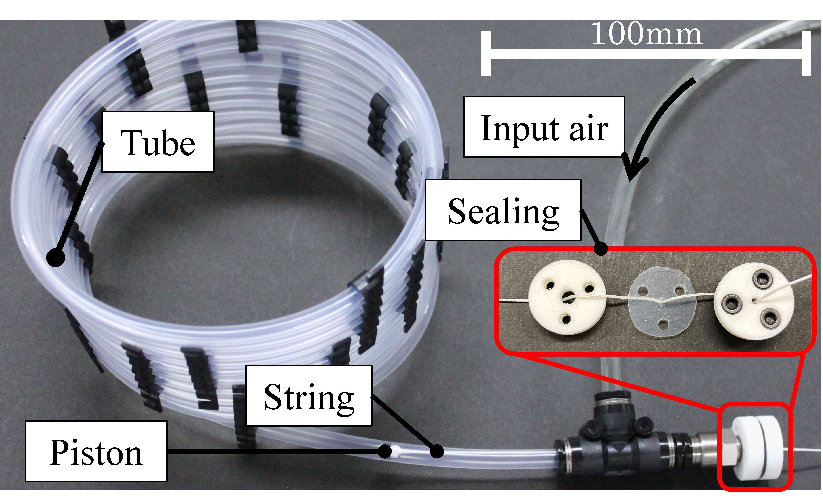
\includegraphics[width=85mm]{_pdf/細径柔軟エアシリンダ-1本.pdf}
  \caption{Air cylinder type artificial muscle}
  \label{Air cylinder type artificial muscle}
\end{figure}

\section{エアシリンダ型人工筋肉の開発}%-----------
\subsection{構造}%-----------
本研究で取り扱うエアシリンダ型人工筋肉とフィッティグの構造を図\ref{Air cylinder type artificial muscle}に示す.シリンダ部分は柔軟チューブ(ニチアス株式会社,材質:ナフロン\textregistered,内外径:$\SI{5}{mm}$, $\SI{6}{mm}$,最小曲げ半径:$\SI{35}{mm}$)である.ロッド部分は紐(ハヤミ工産株式会社,材質:イザナス®,線形:$\SI{0.60}{mm}$,破断強度:$\SI{360}{N}$,破断伸度:$\SI{5.5}{N}$)である.ピストンは2枚のフッ素ゴムリングを2枚のPLA樹脂部品で挟み込む構造である.シール部はゴムシート(材質:NBR,厚さ:1 mm,硬度:70 °(タイプA))である.ゴムシートに穴をあけてロッドを通している.ロッドを通したゴムシートを2つのプラスチック部品をボルトにより挟み込む.

\section{基礎特性の測定}%-----------
エアシリンダ型人工筋肉の各部品間には抵抗力が存在する.1つ目は,シール部と紐の接触による摩擦抵抗$D_s$である.2つ目は,チューブとピストンの接触による摩擦抵抗$D_\mathrm{p}$である.3つ目は,チューブと紐の接触による摩擦抵抗$D_\mathrm{t}$である.抵抗$D_\mathrm{s}$,$D_\mathrm{p}$は印加圧力によって変化すると考えられる.抵抗$D_\mathrm{t}$はチューブと紐の接触角$\theta$によって変化すると考えられる.よって,これら3つの抵抗力$D_\mathrm{s}(P_\mathrm{in})$,$D_\mathrm{p}(P_\mathrm{in})$,$D_\mathrm{t}(\theta)$を実験により測定した.以下に各抵抗$D_\mathrm{s}(P_\mathrm{in})$,$D_\mathrm{p}(P_\mathrm{in})$,$D_\mathrm{t}(\theta)$の実験式を示す.
\begin{align}
  D_\mathrm{s} & = \num{-4.0e-4}P_\mathrm{in} + \num{5.6e-4} \\
  D_\mathrm{p} & = \num{2.1e-3}P_\mathrm{in} + \num{4.0e-4}  \\
  D_\mathrm{t} & = 0.981e^{0.090\theta}
\end{align}


\section{環状に曲がったエアシリンダ型人工筋肉の理論出力}%-----------
\subsection{理論出力の導出}%-----------
柔軟エアシリンダのモデルを図\ref{Model of artifucialmuscle}に示す.人工筋肉は曲率半径$r$で環状に曲がった状態であり,ピストンは巻き角$\theta$の位置にある.巻き角$\theta$,印加圧力$P$における人工筋肉の出力は$F$とする.なお,人工筋肉のロッド直径を$d_\mathrm{string}$,シリンダ内径(ピストン直径)は$d_\mathrm{tube}$である.また,シールとロッドの抵抗力は$D_\mathrm{s}$,シリンダとピストンの抵抗力は$D_\mathrm{p}$である.環状に曲がった人工筋肉においては,従来のエアシリンダでは検討する必要がなかったシリンダとロッドが接触する.モデルにおいては,シリンダとロッドが接触する角度を巻き角$\theta$と仮定する.これらの条件化におけるシリンダとロッドが接触している状態の出力$F$を導出する.
\begin{figure}[t]
  \centering
  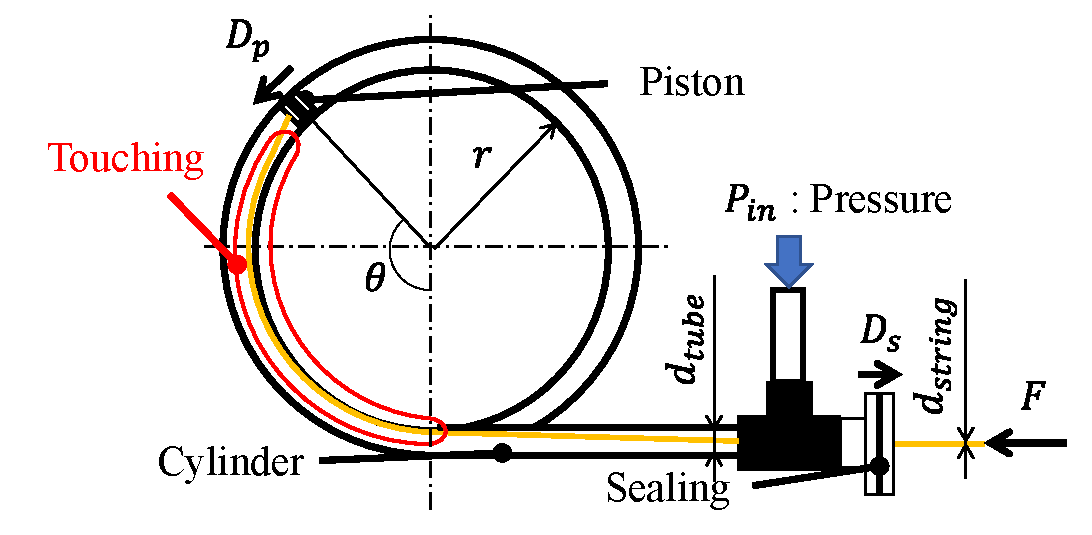
\includegraphics[width=85mm]{_pdf/model_artifucialmuscle.pdf}
  \caption{Model of artifucialmuscle}
  \label{Model of artifucialmuscle}
\end{figure}

シリンダとロッドが接触する場合には,接触部分において摩擦力が生じる.摩擦力によってロッドの先端位置における張力$T_\mathrm{hold}$とピストン位置における張力$T_\mathrm{load}$は異なる.張力$T_\mathrm{hold}$と張力$T_\mathrm{load}$の関係は,キャプスタン方程式よりシリンダとロッドの動摩擦係数$\mu$を用いると,以下のようになる.
\begin{equation}
  \label{T_load}
  T_\mathrm{load}=T_\mathrm{hold}e^{\mu\theta}
\end{equation}
また,ロッド先端における張力$T_\mathrm{hold}$は以下のようになる.
\begin{equation}
  \label{T_hold}
  T_\mathrm{hold}=D_\mathrm{s} + F
\end{equation}
したがって,ピストン位置における張力$T_\mathrm{load}$は式\eqref{T_load},\eqref{T_hold}を用いると,以下のようになる.
\begin{equation}
  \label{T_load_2}
  T_\mathrm{load}=(D_\mathrm{s} + F)e^{\mu\theta}
\end{equation}
次に,ピストン位置におけるつり合いを考える.ピストンにはシリンダとロッドの摩擦による張力$T_\mathrm{load}$,ピストン抵抗$D_\mathrm{p}$,印加圧力$P$によるピストン面圧$F_\mathrm{piston}=\pi/4 \times d_\mathrm{tube}^2 \times P$が加わる.よってピストン位置における張力$T$は以下のようになる.
\begin{equation}
  \label{T}
  T=\frac{\pi}{4}d_\mathrm{tube}^2P-D_\mathrm{p}-(D_\mathrm{s}+F)e^{\mu\theta}
\end{equation}
ピストン位置において力が釣り合うとき,すなわち張力$T=0$のときの出力$F$が人工筋肉の出力となる.したがって,式\eqref{T}へT=0を代入し,変形すると以下のようになる.
\begin{equation}
  \label{F}
  F=\frac{1}{e^{\mu\theta}} (\frac{π}{4}d_\mathrm{tube}^2 P-D_\mathrm{p} )-D_\mathrm{s}
\end{equation}
式\eqref{F}をシリンダとロッドが接触する場合の巻き角$\theta$における人工筋肉の理論出力$F$とする.

\subsection{理論値と実験値の比較}%-----------
巻き角$\theta$における人工筋肉の理論出力$F$と実際の人工筋肉の出力$F$を比較する.理論値と実験値を比較することによって,人工筋肉において起こる現象を明らかにする.
\par
人工筋肉が半径$r$で環状に曲がった状態のピストン位置(巻き角)$θ$における出力$F$を計測する.ロッドの先端をフォースゲージに接続し,人工筋肉に圧力$P$を印可し,出力$F$を測定する.なお,フォースゲージ及びロッドの先端を速度$v=\SI{5}{mm/s}$で直動させる.シリンダの巻き半径$r$は$\SI{100}{mm}$と$\SI{150}{mm}$の2パターンである.印可圧力$P$は$\SI{100}{kPa}~\SI{500}{kPa}$の範囲において$\SI{100}{kPa}$刻みでそれぞれ1回測定を行う.測定終了の判定は,出力$F$が5秒間$\SI{0}{N}$となる場合である.
\par
シリンダの巻き半径$r=\SI{100}{mm}$,$\SI{150}{mm}$の理論値(破線)と実験値(実線)をそれぞれ図\ref{r=100mm},図\ref{r=150mm}に示す.また,実験値は区間1000で移動平均を実施した.図\ref{r=100mm},\ref{r=150mm}より,巻き角$\theta=0 \sim 2\pi$までは実験値が理論値よりも高いことが示されている.この原因は,曲がったシリンダに対するピストン抵抗力$D_\mathrm{p}$は,ピストンがまっすぐな抵抗力$D_\mathrm{p}$よりも小さくなったためである.理論出力$F$の導出に用いたピストン抵抗力$D_\mathrm{p}$は,ピストンのワッシャ側面がシリンダに完全接触している条件である.しかし,シリンダが曲がった状態では,ピストンのワッシャ側面が完全に接触しない.したがって,曲がったシリンダにおけるピストン抵抗力$D_\mathrm{p}$は3.1.3節で測定した抵抗力$D_\mathrm{p}$よりも小さくなり,実際の出力$F$が理論値よりも大きくなったと考えられる.また,巻き角$\theta=2\pi$以降はおおむね実験値が理論値よりも低いことが示されている.巻き角$\theta=2\pi$すなわちロッドがシリンダを一周したときに,シリンダの巻き半径$r$を小さくするような力が働く.この力によりシリンダがわずかに変形し,変形量の分,出力$F$が低下したと考えられる.また,図\ref{r=100mm}と図\ref{r=150mm}より,巻き半径$r=\SI{100}{mm}$の実験値のほうが$r=\SI{150}{mm}$より大きいことがわかる.
\begin{figure}[t]
  \centering
  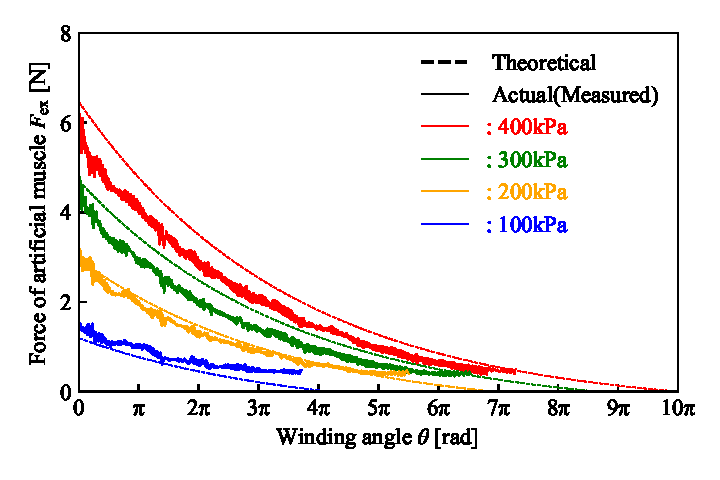
\includegraphics[width=85mm]{_pdf/result_100mm.pdf}
  \caption{Result of winding radius $r=100$}
  \label{r=100mm}
\end{figure}

\begin{figure}[t]
  \centering
  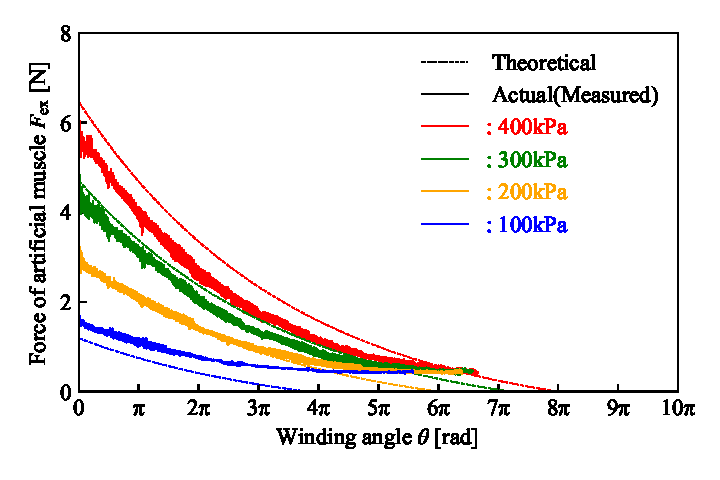
\includegraphics[width=85mm]{_pdf/result_150mm.pdf}
  \caption{Result of winding radius $r=150$}
  \label{r=150mm}
\end{figure}

\section{エアシリンダ型人工筋肉を用いた揺動アームの開発}%-----------
\subsection{揺動アームの構造}
エアシリンダ型人工筋肉を機械要素として応用する方法を検討する.機械要素として応用する場合には,エアシリンダ型人工筋肉の本数や配置を設計および制御方法について検討する必要がある.そこで,エアシリンダ型人工筋肉を揺動アームに4本取り付け,アームの角度を制御する.図\ref{Swing arm}に揺動アームの概要を示す.エアシリンダ型人工筋肉はアームに対し対抗配置(2本×2セット)する.なお,エアシリンダ型人工筋肉の印加圧力は2系統であり,それぞれ圧力$P_\mathrm{a}$,$P_\mathrm{b}$とする.また,揺動アーム根本に取り付けたプーリによりエアシリンダ型人工筋肉の直動運動を回転運動に変換する.アームの揺動角度を$\theta$とし,アームに取り付けた3軸ジャイロ+3軸加速度センサにより角度$\theta$を計測する.
\begin{figure}[t]
  \centering
  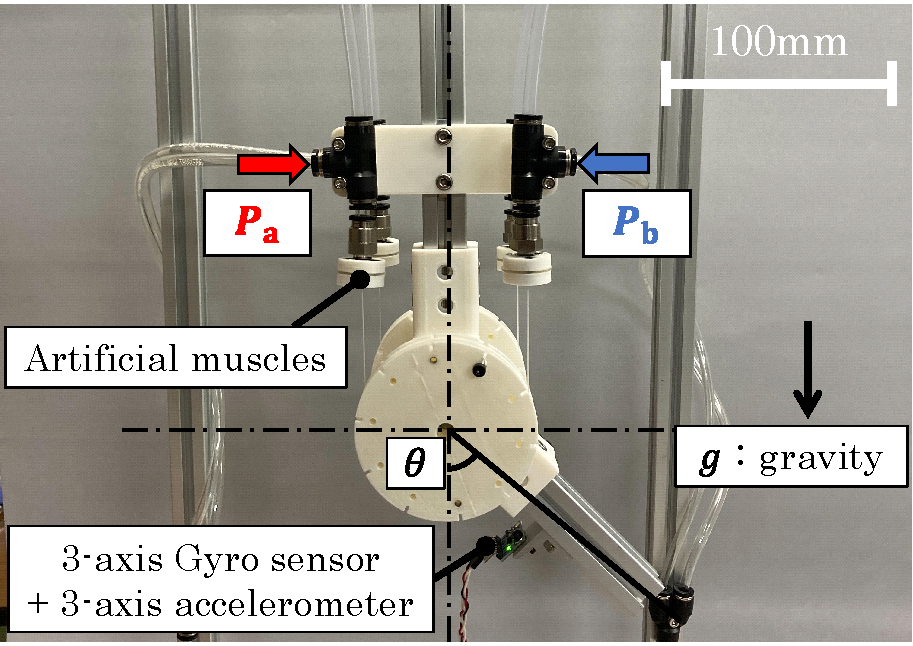
\includegraphics[width=85mm]{_pdf/swing_arm.pdf}
  \caption{Swing arm}
  \label{Swing arm}
\end{figure}

\subsection{揺動アームの角度制御}
目標値を揺動アームの角度$\theta$とした場合の,制御性について評価を行う.制御方法は2系統の印加圧力の平均$P_\mathrm{ave}=(P_\mathrm{a} + P_\mathrm{b})/2$を一定値として入力し,差圧$\Delta P = P_\mathrm{a} - P_\mathrm{b}$を制御値とする.目標値は$\theta_p = 90 \sin(0.01t)$とし,実角度$\theta$を測定する.なお,エアシリンダ型人工筋肉のチューブは真っすぐな状態で測定を行った.
\par
図~に測定結果を示す.・・・
\section{結言}%-----------
・・・